Blake2~\cite{blake2} is a cryptographic hash and \gls{mac}. It is faster than
\emph{MD5}, \emph{SHA-1}, \emph{SHA-2} and \emph{SHA-3}, but is at least as
secure as the latest standard \emph{SHA-3}.
It comes in two flavors:
\begin{itemize}
	\item \emph{Blake2B} is optimised for $64$-bit platforms and produces
		digests of any size between $1$ and $64$ bytes
	\item \emph{Blake2S} is optimised for $8$- to $32$-bit platforms and
		produces digests of any size between $1$ and $32$ bytes.
\end{itemize}

A hardware implementation was created by Benedikt Tutzer and Dinka Milovancev as
part of the \emph{Digital Integrated Circuits} Laboratory at TU
Wien~\cite{blake2hardware}.
Although a 32-bit platform is used, it was decided to implement Blake2B, as it is possible to choose which bit-width should be used at the hardware level.

Since this IP core was already created in the previous project \cite{oldrepo}, the core is added to the system design as described in
\cref{ssec:zynqhardwaredesign} and given the address $0x88000000$. A size of
$64K$ is sufficient.

All needed files of the IP core can be found in \emph{<repo>/hardware\_design/ip_repo/blake2b\_v1\_00\_a}.
The files from~\cite{blake2hardware} are located at the vhdl-source directory
of the core,\\
\emph{<repo>/hardware\_design/ip_repo/blake2b\_v1\_00\_a/hdl/vhdl}.

The IP core was configured to have $4$ software accessible registers, each $32$-bit wide:

\begin{tabular}{ll}
	Address & Name \\
	base     & task\_reg\\
	base + 4 & message\_reg\\
	base + 8 & status\_reg\\
	base + 16 & hash\_reg\\
\end{tabular}
\medbreak

With interface generated by the Xilinx tools, the core is only able to react to
register reads or -writes from the software.
It cannot send interrupts to the software.
To add this functionality, an additional port, of type \emph{std\_logic} is
added and routed through the wrapper in \emph{blake2b.vhd} so that it is
visible as an output port of the peripheral.
It is called \emph{Interrupt}.

The port shows up as an interrupt port.
To connect it to the \gls{gic}, the port must be connected to the platform interrupt input of the Zynq. 
\Cref{fig:hwsystem} shows the Vivado block design of the system.

\begin{figure}[htbp]
    \centering
    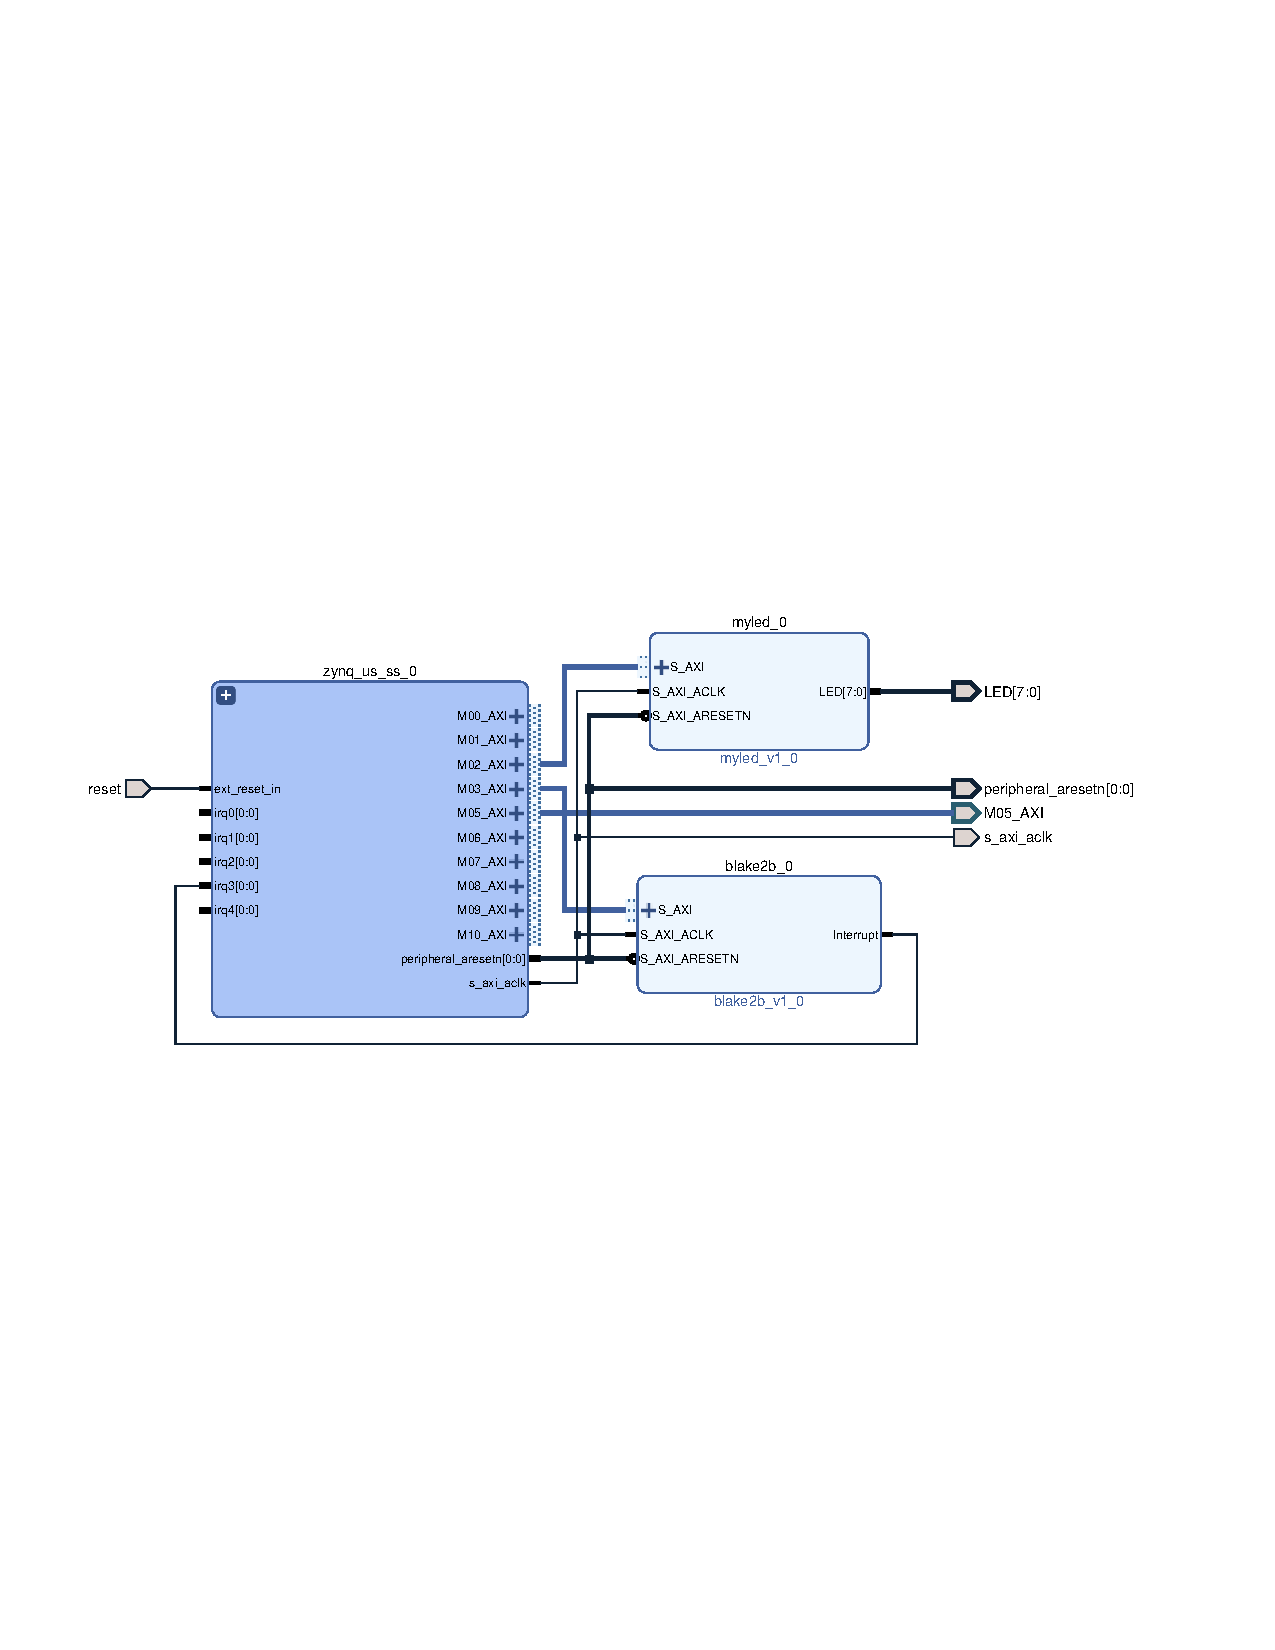
\includegraphics[width=1\textwidth]{images/hw-design-system.png}
    \caption{\label{fig:hwsystem} Vivado block design of the system}
\end{figure}

The protocol how this device communicates with the device driver is simple.
To hash data, it has to be split into chunks of $32$-bits as the registers are
only $32$ bits wide.
The following steps need to be followed to hash data:
\begin{enumerate}
	\item Driver writes number of bytes to be hashed to the task register
	\item If all the data was sent, go to \Cref{item:end}\label{item:check}
	\item Device raises interrupt to signal that more data is needed
	\item Driver catches interrupt and writes a chunk of data to the message
		register
	\item Go to \Cref{item:check}
	\item Device raises interrupt to signal that hashing is done\label{item:end}
\end{enumerate}
The hash is always $64$-bytes long, so to read it back to the driver it has to
be split into $16$ individual $32$-bit chunks.
To read the hash from the device, the following steps are done:
\begin{enumerate}
	\item Driver iterates over $16$ hash chunks
		\begin{enumerate}
			\item Driver writes index of hash-chunk to status register
			\item Devices places the according chunk onto the hash register
			\item Driver reads hash register
		\end{enumerate}
	\item Driver concatenates hash chunks
\end{enumerate}
